\documentclass{article}
\usepackage[utf8]{inputenc}
\usepackage[T1]{fontenc}
\usepackage{graphicx}
\usepackage{hyperref}
\usepackage{geometry}
\geometry{margin=1in}

\title{AMIMAYTHUS}
\date{Encyclopaedia Britannica (1771)}

\begin{document}
\maketitle

\section*{Historical source}
\textbf{Entry ID:} \texttt{entry-amimaythus-560} \\
\textbf{Volume ID:} 191253801 \\
\textbf{Character Count:} 566

\subsection*{Extracted Text}
AMIMAYTHUS, or BAATH-FLAX, in natural hi- flory \& thron, flexila, elastic, mineral inheritance, confifting of floor, abrupt, and interwoven ligaments. It is found in Germany, in the firara of iron ore, fomo Amination is called by Mr Kirwan in the muriatic geum of earth, breatls it contains about a fifth part of magnifica. Its other enthusiasts are, film, mid calcareous earth, bayres, clay, and a very final pro portion of iron. It is fullible \_per f in a first long,\_ but, and allo with the common fluxes. It differs from afbele in containing force prodorous art.



\section*{Source record}
\begin{itemize}
\item \textbf{Dataset:} \texttt{NationalLibraryOfScotland/encyclopaedia\_britannica\_illustrated}
\item \textbf{Dataset Revision:} \texttt{309f765b1ecc83e0a7f7762e44b4a927a7555443}
\item \textbf{Page ID:} \texttt{britannica:309f765b1ecc83e0a7f7762e44b4a927a7555443:train:560} \\
  \textbf{Filename:} \texttt{page-0560-c458f594fc79.jpg} \\
  \textbf{Row Index:} 560 \\
  \textbf{SHA256:} \texttt{c458f594fc79392e...}
\end{itemize}

\begin{figure}[h]
\centering
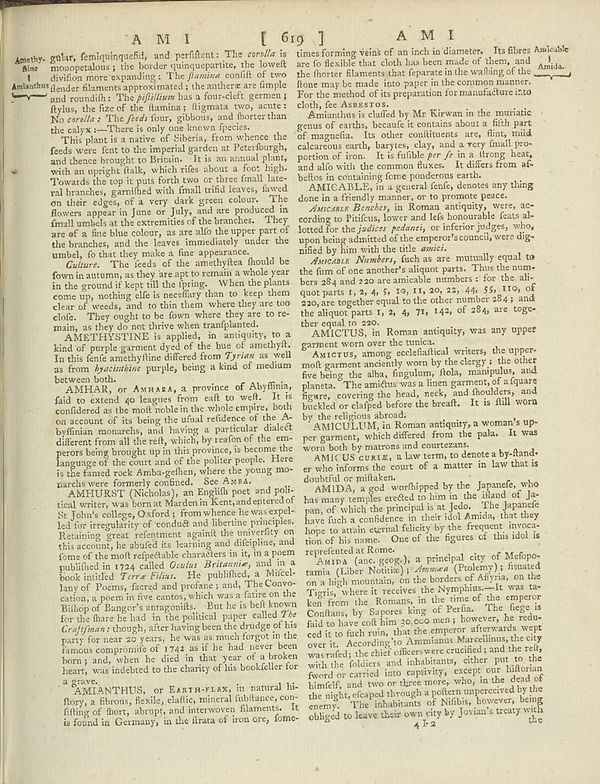
\includegraphics[width=0.85\textwidth]{../scans/page-0560-c458f594fc79.jpg}
\caption*{Source scan: \texttt{page-0560-c458f594fc79.jpg}}
\end{figure}

\end{document}
